
%% bare_conf.tex
%% V1.4b
%% 2015/08/26
%% by Michael Shell
%% See:
%% http://www.michaelshell.org/
%% for current contact information.
%%
%% This is a skeleton file demonstrating the use of IEEEtran.cls
%% (requires IEEEtran.cls version 1.8b or later) with an IEEE
%% conference paper.
%%
%% Support sites:
%% http://www.michaelshell.org/tex/ieeetran/
%% http://www.ctan.org/pkg/ieeetran
%% and
%% http://www.ieee.org/

%%*************************************************************************
%% Legal Notice:
%% This code is offered as-is without any warranty either expressed or
%% implied; without even the implied warranty of MERCHANTABILITY or
%% FITNESS FOR A PARTICULAR PURPOSE! 
%% User assumes all risk.
%% In no event shall the IEEE or any contributor to this code be liable for
%% any damages or losses, including, but not limited to, incidental,
%% consequential, or any other damages, resulting from the use or misuse
%% of any information contained here.
%%
%% All comments are the opinions of their respective authors and are not
%% necessarily endorsed by the IEEE.
%%
%% This work is distributed under the LaTeX Project Public License (LPPL)
%% ( http://www.latex-project.org/ ) version 1.3, and may be freely used,
%% distributed and modified. A copy of the LPPL, version 1.3, is included
%% in the base LaTeX documentation of all distributions of LaTeX released
%% 2003/12/01 or later.
%% Retain all contribution notices and credits.
%% ** Modified files should be clearly indicated as such, including  **
%% ** renaming them and changing author support contact information. **
%%*************************************************************************


% *** Authors should verify (and, if needed, correct) their LaTeX system  ***
% *** with the testflow diagnostic prior to trusting their LaTeX platform ***
% *** with production work. The IEEE's font choices and paper sizes can   ***
% *** trigger bugs that do not appear when using other class files.       ***
% The testflow support page is at:
% http://www.michaelshell.org/tex/testflow/



\documentclass[conference]{IEEEtran}
% Some Computer Society conferences also require the compsoc mode option,
% but others use the standard conference format.
%
% If IEEEtran.cls has not been installed into the LaTeX system files,
% manually specify the path to it like:
% \documentclass[conference]{../sty/IEEEtran}





% Some very useful LaTeX packages include:
% (uncomment the ones you want to load)


% *** MISC UTILITY PACKAGES ***
%
%\usepackage{ifpdf}
% Heiko Oberdiek's ifpdf.sty is very useful if you need conditional
% compilation based on whether the output is pdf or dvi.
% usage:
% \ifpdf
%   % pdf code
% \else
%   % dvi code
% \fi
% The latest version of ifpdf.sty can be obtained from:
% http://www.ctan.org/pkg/ifpdf
% Also, note that IEEEtran.cls V1.7 and later provides a builtin
% \ifCLASSINFOpdf conditional that works the same way.
% When switching from latex to pdflatex and vice-versa, the compiler may
% have to be run twice to clear warning/error messages.






% *** CITATION PACKAGES ***
%
%\usepackage{cite}
% cite.sty was written by Donald Arseneau
% V1.6 and later of IEEEtran pre-defines the format of the cite.sty package
% \cite{} output to follow that of the IEEE. Loading the cite package will
% result in citation numbers being automatically sorted and properly
% "compressed/ranged". e.g., [1], [9], [2], [7], [5], [6] without using
% cite.sty will become [1], [2], [5]--[7], [9] using cite.sty. cite.sty's
% \cite will automatically add leading space, if needed. Use cite.sty's
% noadjust option (cite.sty V3.8 and later) if you want to turn this off
% such as if a citation ever needs to be enclosed in parenthesis.
% cite.sty is already installed on most LaTeX systems. Be sure and use
% version 5.0 (2009-03-20) and later if using hyperref.sty.
% The latest version can be obtained at:
% http://www.ctan.org/pkg/cite
% The documentation is contained in the cite.sty file itself.
\usepackage[style=ieee]{biblatex}
\addbibresource{../thesis/references.bib} 

\usepackage{csquotes}
\usepackage{cleveref}
\usepackage{subcaption}

\usepackage{amsmath}
\usepackage{amssymb}
\usepackage{amsthm}

\usepackage{algorithm}
\usepackage[noend]{algpseudocode} 
\algnewcommand\algorithmicupon{\textbf{Upon}}
\algnewcommand\Upon{\item[\algorithmicupon]}

\algnewcommand\algorithmicsend{\textbf{Send}}
\algnewcommand\Send{\item[\algorithmicsend]}

\DeclareMathOperator*{\argmin}{arg\,min}

\theoremstyle{plain}
\newtheorem{theorem}{Theorem}
\newtheorem{corollary}{Corollary}
\newtheorem{lemma}{Lemma}
\newtheorem{claim}{Claim}
\newtheorem{definition}{Definition}

\newcommand{\A}{\mathcal{A}}
\newcommand{\C}{\mathcal{C}}
\renewcommand{\P}{\mathcal{P}}
\newcommand{\F}{\mathcal{F}}
\newcommand{\E}{\mathcal{E}}



% *** GRAPHICS RELATED PACKAGES ***
%
\ifCLASSINFOpdf
  \usepackage[pdftex]{graphicx}
  % declare the path(s) where your graphic files are
  \graphicspath{{../figures/}}
  % and their extensions so you won't have to specify these with
  % every instance of \includegraphics
  % \DeclareGraphicsExtensions{.pdf,.jpeg,.png}
\else
  % or other class option (dvipsone, dvipdf, if not using dvips). graphicx
  % will default to the driver specified in the system graphics.cfg if no
  % driver is specified.
  \usepackage[dvips]{graphicx}
  % declare the path(s) where your graphic files are
  \graphicspath{{../figures/}}
  % and their extensions so you won't have to specify these with
  % every instance of \includegraphics
  % \DeclareGraphicsExtensions{.eps}
\fi
% graphicx was written by David Carlisle and Sebastian Rahtz. It is
% required if you want graphics, photos, etc. graphicx.sty is already
% installed on most LaTeX systems. The latest version and documentation
% can be obtained at: 
% http://www.ctan.org/pkg/graphicx
% Another good source of documentation is "Using Imported Graphics in
% LaTeX2e" by Keith Reckdahl which can be found at:
% http://www.ctan.org/pkg/epslatex
%
% latex, and pdflatex in dvi mode, support graphics in encapsulated
% postscript (.eps) format. pdflatex in pdf mode supports graphics
% in .pdf, .jpeg, .png and .mps (metapost) formats. Users should ensure
% that all non-photo figures use a vector format (.eps, .pdf, .mps) and
% not a bitmapped formats (.jpeg, .png). The IEEE frowns on bitmapped formats
% which can result in "jaggedy"/blurry rendering of lines and letters as
% well as large increases in file sizes.
%
% You can find documentation about the pdfTeX application at:
% http://www.tug.org/applications/pdftex





% *** MATH PACKAGES ***
%
%\usepackage{amsmath}
% A popular package from the American Mathematical Society that provides
% many useful and powerful commands for dealing with mathematics.
%
% Note that the amsmath package sets \interdisplaylinepenalty to 10000
% thus preventing page breaks from occurring within multiline equations. Use:
%\interdisplaylinepenalty=2500
% after loading amsmath to restore such page breaks as IEEEtran.cls normally
% does. amsmath.sty is already installed on most LaTeX systems. The latest
% version and documentation can be obtained at:
% http://www.ctan.org/pkg/amsmath





% *** SPECIALIZED LIST PACKAGES ***
%
%\usepackage{algorithmic}
% algorithmic.sty was written by Peter Williams and Rogerio Brito.
% This package provides an algorithmic environment fo describing algorithms.
% You can use the algorithmic environment in-text or within a figure
% environment to provide for a floating algorithm. Do NOT use the algorithm
% floating environment provided by algorithm.sty (by the same authors) or
% algorithm2e.sty (by Christophe Fiorio) as the IEEE does not use dedicated
% algorithm float types and packages that provide these will not provide
% correct IEEE style captions. The latest version and documentation of
% algorithmic.sty can be obtained at:
% http://www.ctan.org/pkg/algorithms
% Also of interest may be the (relatively newer and more customizable)
% algorithmicx.sty package by Szasz Janos:
% http://www.ctan.org/pkg/algorithmicx




% *** ALIGNMENT PACKAGES ***
%
%\usepackage{array}
% Frank Mittelbach's and David Carlisle's array.sty patches and improves
% the standard LaTeX2e array and tabular environments to provide better
% appearance and additional user controls. As the default LaTeX2e table
% generation code is lacking to the point of almost being broken with
% respect to the quality of the end results, all users are strongly
% advised to use an enhanced (at the very least that provided by array.sty)
% set of table tools. array.sty is already installed on most systems. The
% latest version and documentation can be obtained at:
% http://www.ctan.org/pkg/array


% IEEEtran contains the IEEEeqnarray family of commands that can be used to
% generate multiline equations as well as matrices, tables, etc., of high
% quality.




% *** SUBFIGURE PACKAGES ***
%\ifCLASSOPTIONcompsoc
%  \usepackage[caption=false,font=normalsize,labelfont=sf,textfont=sf]{subfig}
%\else
%  \usepackage[caption=false,font=footnotesize]{subfig}
%\fi
% subfig.sty, written by Steven Douglas Cochran, is the modern replacement
% for subfigure.sty, the latter of which is no longer maintained and is
% incompatible with some LaTeX packages including fixltx2e. However,
% subfig.sty requires and automatically loads Axel Sommerfeldt's caption.sty
% which will override IEEEtran.cls' handling of captions and this will result
% in non-IEEE style figure/table captions. To prevent this problem, be sure
% and invoke subfig.sty's "caption=false" package option (available since
% subfig.sty version 1.3, 2005/06/28) as this is will preserve IEEEtran.cls
% handling of captions.
% Note that the Computer Society format requires a larger sans serif font
% than the serif footnote size font used in traditional IEEE formatting
% and thus the need to invoke different subfig.sty package options depending
% on whether compsoc mode has been enabled.
%
% The latest version and documentation of subfig.sty can be obtained at:
% http://www.ctan.org/pkg/subfig




% *** FLOAT PACKAGES ***
%
%\usepackage{fixltx2e}
% fixltx2e, the successor to the earlier fix2col.sty, was written by
% Frank Mittelbach and David Carlisle. This package corrects a few problems
% in the LaTeX2e kernel, the most notable of which is that in current
% LaTeX2e releases, the ordering of single and double column floats is not
% guaranteed to be preserved. Thus, an unpatched LaTeX2e can allow a
% single column figure to be placed prior to an earlier double column
% figure.
% Be aware that LaTeX2e kernels dated 2015 and later have fixltx2e.sty's
% corrections already built into the system in which case a warning will
% be issued if an attempt is made to load fixltx2e.sty as it is no longer
% needed.
% The latest version and documentation can be found at:
% http://www.ctan.org/pkg/fixltx2e


%\usepackage{stfloats}
% stfloats.sty was written by Sigitas Tolusis. This package gives LaTeX2e
% the ability to do double column floats at the bottom of the page as well
% as the top. (e.g., "\begin{figure*}[!b]" is not normally possible in
% LaTeX2e). It also provides a command:
%\fnbelowfloat
% to enable the placement of footnotes below bottom floats (the standard
% LaTeX2e kernel puts them above bottom floats). This is an invasive package
% which rewrites many portions of the LaTeX2e float routines. It may not work
% with other packages that modify the LaTeX2e float routines. The latest
% version and documentation can be obtained at:
% http://www.ctan.org/pkg/stfloats
% Do not use the stfloats baselinefloat ability as the IEEE does not allow
% \baselineskip to stretch. Authors submitting work to the IEEE should note
% that the IEEE rarely uses double column equations and that authors should try
% to avoid such use. Do not be tempted to use the cuted.sty or midfloat.sty
% packages (also by Sigitas Tolusis) as the IEEE does not format its papers in
% such ways.
% Do not attempt to use stfloats with fixltx2e as they are incompatible.
% Instead, use Morten Hogholm'a dblfloatfix which combines the features
% of both fixltx2e and stfloats:
%
% \usepackage{dblfloatfix}
% The latest version can be found at:
% http://www.ctan.org/pkg/dblfloatfix




% *** PDF, URL AND HYPERLINK PACKAGES ***
%
%\usepackage{url}
% url.sty was written by Donald Arseneau. It provides better support for
% handling and breaking URLs. url.sty is already installed on most LaTeX
% systems. The latest version and documentation can be obtained at:
% http://www.ctan.org/pkg/url
% Basically, \url{my_url_here}.




% *** Do not adjust lengths that control margins, column widths, etc. ***
% *** Do not use packages that alter fonts (such as pslatex).         ***
% There should be no need to do such things with IEEEtran.cls V1.6 and later.
% (Unless specifically asked to do so by the journal or conference you plan
% to submit to, of course. )


% correct bad hyphenation here
\hyphenation{op-tical net-works semi-conduc-tor block-chain crypto-currency}

\IEEEoverridecommandlockouts
\IEEEpubid{%
   \makebox[\columnwidth]{ISBN 978-3-903176-08-9~\copyright~2018 IFIP \hfill}%
   \hspace{\columnsep}% 
   \makebox[\columnwidth]{ }% 
}

\begin{document}
%
% paper title
% Titles are generally capitalized except for words such as a, an, and, as,
% at, but, by, for, in, nor, of, on, or, the, to and up, which are usually
% not capitalized unless they are the first or last word of the title.
% Linebreaks \\ can be used within to get better formatting as desired.
% Do not put math or special symbols in the title.
\title{A Blockchain Consensus Protocol With\\Horizontal Scalability}


% author names and affiliations
% use a multiple column layout for up to three different
% affiliations
\author{\IEEEauthorblockN{Kelong Cong}
\IEEEauthorblockA{\'{E}cole Polytechnique F\'{e}d\'{e}rale de Lausanne\\
Email: kelong.cong@epfl.ch}
\and
\IEEEauthorblockN{Zhijie Ren}
\IEEEauthorblockA{Delft University of Technology\\
Email: z.ren@tudelft.nl}
\and
\IEEEauthorblockN{Johan Pouwelse}
\IEEEauthorblockA{Delft University of Technology\\
Email: peer2peer@gmail.com}
}

% conference papers do not typically use \thanks and this command
% is locked out in conference mode. If really needed, such as for
% the acknowledgment of grants, issue a \IEEEoverridecommandlockouts
% after \documentclass

% for over three affiliations, or if they all won't fit within the width
% of the page, use this alternative format:
% 
%\author{\IEEEauthorblockN{Michael Shell\IEEEauthorrefmark{1},
%Homer Simpson\IEEEauthorrefmark{2},
%James Kirk\IEEEauthorrefmark{3}, 
%Montgomery Scott\IEEEauthorrefmark{3} and
%Eldon Tyrell\IEEEauthorrefmark{4}}
%\IEEEauthorblockA{\IEEEauthorrefmark{1}School of Electrical and Computer Engineering\\
%Georgia Institute of Technology,
%Atlanta, Georgia 30332--0250\\ Email: see http://www.michaelshell.org/contact.html}
%\IEEEauthorblockA{\IEEEauthorrefmark{2}Twentieth Century Fox, Springfield, USA\\
%Email: homer@thesimpsons.com}
%\IEEEauthorblockA{\IEEEauthorrefmark{3}Starfleet Academy, San Francisco, California 96678-2391\\
%Telephone: (800) 555--1212, Fax: (888) 555--1212}
%\IEEEauthorblockA{\IEEEauthorrefmark{4}Tyrell Inc., 123 Replicant Street, Los Angeles, California 90210--4321}}




% use for special paper notices
%\IEEEspecialpapernotice{(Invited Paper)}


% make the title area
\maketitle
%\thispagestyle{plain}
\pagestyle{plain}

% switch off page numbers
\pagenumbering{gobble}

% As a general rule, do not put math, special symbols or citations
% in the abstract
\begin{abstract}
Blockchain technology has the potential to decentralise many traditionally centralised systems.
However, scalability remains a key challenge.
A horizontally scalable solution,
where performance increases by adding more nodes,
would move blockchain systems one step closer to ubiquitous use.
% what's the solution?
We design a novel blockchain system called \textsc{Checo}.
Each node in our system maintains a personal hash chain,
which only stores transactions that the node is involved in.
A consensus is reached on special blocks called checkpoint blocks rather than on all transactions.
Checkpoint blocks are effectively a hash pointer to the personal hash chains;
thus a single checkpoint block may represent an arbitrarily large set of transactions.
We introduce a validation protocol so that any node can check the validity of any transaction.
Since transaction and validation protocols are point-to-point, we achieve horizontal scalability.
% how good is the solution?
We analytically evaluate our system and show a number of highly desirable correctness properties such as consensus on the validity of transactions.
Further, we give a free and open-source implementation of \textsc{Checo} and evaluate it experimentally.
Our results show a strong indication of horizontal scalability.
\end{abstract}

% no keywords




% For peer review papers, you can put extra information on the cover
% page as needed:
% \ifCLASSOPTIONpeerreview
% \begin{center} \bfseries EDICS Category: 3-BBND \end{center}
% \fi
%
% For peerreview papers, this IEEEtran command inserts a page break and
% creates the second title. It will be ignored for other modes.
\IEEEpeerreviewmaketitle



\section{Introduction}

% problem description
Bitcoin is almost 10 years old and its market capitalisation is over \$60 billion USD and growing~\cite{bitcoinmarketcap}.
We can be reasonably sure that cryptocurrencies,
even if their application is still somewhat limited,
are here to stay in the foreseeable future.
Driven by the success of Bitcoin, we are seeing a renaissance of consensus research~\cite{miller2016honey, kogias2016enhancing, kokoris2017omniledger},
where the primary focus is to improve the scalability of blockchain system.
This is due to the inefficiencies in the consensus mechanism in early blockchain systems---proof-of-work (PoW).
For example, Bitcoin can only do 7 transactions per second (TPS) at most~\cite{vukolic2015quest}.
While adjusting the block size (which Bitcoin has recently done via SegWit~\cite{segwit}) and/or the block interval may increase TPS,
it also leads to centralisation as larger blocks take longer to propagate in the network,
giving miners that do not have a fast network a disadvantage~\cite{croman2016scaling}.
In today's network, it is not possible to achieve more than 758 TPS
if new blocks need to be propogated timely to 90\% of the network~\cite{croman2016scaling}.

% related work
Many approaches exist for improving the scalability of early blockchains.
Off-chain transactions make use of the fact that if nodes make frequent transactions,
then it is not necessary to store every transaction on the blockchain,
only the net settlement is necessary.
The best examples are Lightning Network~\cite{lightningnetwork} and Duplex Micropayment Channels~\cite{decker2015fast}.
It promises significant scalability improvements,
but complicates user experience and heavily relies on the semantics of transactions.
Each node must deposit a suitable amount of Bitcoins into a multi-signature account.
A low deposit would not allow large transactions.
A high deposit locks the user from using much of her Bitcoins outside the channel.
In addition, the user must proactively check whether the counterparty has broadcasted an old channel state so that the user does not lose Bitcoins.
Payment channel, in theory, solves the scalability problem of early blockchain systems,
but to the best of our knowledge, its exact scalability characteristics are not investigated.

Another way to improve transaction rate is to use traditional Byzantine consensus algorithms such as PBFT~\cite{castro1999practical}.
In essence, they contain a fixed set of nodes (sometimes called validating peer) that run a Byzantine consensus algorithm to decide on new blocks.
This is often used in permissioned system where the validators must be predetermined, e.g. Hyperledger Fabric~\cite{cachin2016architecture}.
Such systems can achieve much higher transaction rates, e.g. 10,000 TX/s if the number of validating peer is under 16 for PBFT~\cite[Section 5.2]{miller2016honey}.
However, these systems do not scale, e.g. the transaction rate drops to under 5000 TX/s when the number of validating peer is 64~\cite[Section 5.2]{miller2016honey}.
Moreover, the validating peers are predetermined which makes the system unsuitable for the open internet.

Recent research has developed a class of hybrid systems which uses PoW for committee election,
and Byzantine consensus algorithms to agree on transactions, e.g. SCP~\cite{luu2015scp}, ByzCoin~\cite{kogias2016enhancing} and Solidus~\cite{abraham2016solidus}.
This design is primarily for permissionless system because the PoW leader election aspect prevents Sybils.
This technique overcomes the early blockchain scalability issue by delegating the transaction validation to the Byzantine consensus protocol (e.g. PBFT in ByzCoin~\cite{kogias2016enhancing}).
A major tradeoff of such systems is that they cannot guarantee correctness when there is a large number of malicious nodes (but less than a majority).
For SCP, ByzCoin and Solidus, they all have some probability to elect more than $t$ Byzantine nodes into the committee,
where $t$ is typically just under a third of the committee size (a lower bound of Byzantine consensus~\cite{pease1980reaching}).
This problem is especially difficult to solve because the committee is always much smaller than the population size which has more than $t$ Byzantine nodes.
Again, due to the fact that these systems must reach consensus on all transactions,
none of them achieves horizontal scalability.

Finally, a technique that does achieve horizontal scalability is sharding, e.g. Elastico~\cite{luu2016elastico} and OmniLedger~\cite{kokoris2017omniledger}.
This is done by grouping nodes into multiple committees or shards of constant size.
Nodes within a single shard run a Byzantine consensus algorithm to agree on a set of transactions that belong to that specific shard.
The number of shards grows linearly with respect to the total computational power in the network, hence the transaction rate also grows linearly.
The biggest limitation of sharding is that it is only optimal is transactions stay in the same shard.
In fact, Elastico cannot atomically process inter-shard transactions.
OmniLedger has an inter-shard transaction protocol but choosing a good shard size is difficult.
A large shard size would make the system less scalable because the Byzantine consensus algorithm must be run by a large number of nodes.
A small shard size would result in a large number of inter-shard transactions which also hinder scalability.
The authors of OmniLedger noted that inter-shard transactions have significantly higher latency compared to the consensus protocol~\cite{kokoris2017omniledger}.

% research question
In this work, answer the following research question.
\begin{displayquote}
\emph{Is it possible to design a blockchain consensus protocol that is fault-tolerant and horizontally scalable?}
\end{displayquote}
A blockchain consensus protocol should be application neutural,
for example PoW without the transaction logic.
Our system should be Byzantine fault tolerant up to some threshold.
The threshold may be made adjustable by trading off performance.
Finally, we are interested in horizontal scalability in the general case, as it enables ubiquitous use.
That is, by adding new nodes into the network, the global transaction rate should increase proportionally.

% contribution
The key insight is to \emph{not} reach consensus using an existing consensus algorithm (a modified HoneyBadgerBFT~\cite{miller2016honey}) on transactions themselves but on special blocks called checkpoint blocks,
such that transactions are nevertheless verifiable at a later stage by any node in the network.
Our main contributions are the following.
\begin{itemize}
    \item We formally introduce a blockchain system---\textsc{Checo}\footnote{\emph{Che}ckpoint \emph{co}nsensus}.
        It uses individual hash chains and checkpoints on every node to achieve
        horizontally scalable for the first time.
    \item We analyse \textsc{Checo} to ensure correctness as defined in our architecture.
    \item We provide an implementation and then experiment with up to 1200 nodes,
        our results show strong evidence of horizontal scalability.
\end{itemize}

% organisation
In~\Cref{sec:description},
we give the problem description and our system model.
\Cref{sec:system} gives the formal system architecture.
Next, we argue the correctness and fault tolerance properties of our system in~\Cref{sec:analysis}.
We evaluate our system experimentally in~\Cref{sec:implementation}.
Finally, we conclude our work in~\Cref{sec:conclusion}.

\section{Problem Description}
\label{sec:description}
We introduce the problem as a modified Byzantine consensus problem.
In our model, we consider $N$ nodes, $t$ of which are Byzantine.
Nodes in our system make transactions with each other.
Transactions can be in one of three states---\emph{valid}, \emph{invalid} and \emph{unknown}, defined by some function $\textsf{get\_validity}(\cdot)$.
We seek a protocol that reasonably defines these states given a transaction,
but also satisfies the following properties.
\begin{itemize}
    \item \emph{Agreement}:
        If any correct node decides on the validity (except when it is \emph{unknown}) of a transaction,
        then all other correct nodes are able to reach the same conclusion or \emph{unknown}.
    \item \emph{Validity}:
        The protocol outputs the correct result according to $\textsf{get\_validity}(\cdot).$
    \item \emph{Scalability}:
        If every node makes transactions at the same rate,
        then as $N$ increases,
        the global transaction rate should increase linearly w.r.t. $N$.
\end{itemize}

Note that the agreement and validity property are similar to what is often seen in Byzantine consensus problems,
but there are subtle differences and relaxations.
Firstly, the agreement property only holds if honest nodes do not output \emph{unknown}.
For example, for a transaction, it is OK if two honest nodes output \emph{valid} and \emph{unknown}, but it is not OK to output \emph{valid} and \emph{invalid}.
Secondly, the validity is a relaxation of what is typically seen in Byzantine consensus problems,
namely we do not make any guarantee on whether the transaction is \emph{valid} even if all nodes are honest,
only that it is correct according to $\textsf{get\_validity}(\cdot)$ defined by the protocol.

The problem is purposefully made to be application neutral,
i.e. there are no constraints on the semantics of transactions.
This is so that the protocol can act as a backbone to many applications.
Due to this fact, we also do not consider global fork prevention or detection,
as some application may not need such strong guarantees such as recording the number of bytes uploaded and downloaded in Tribler~\cite{pimotte, pouwelse2008tribler}.
On the other hand, we give two alternative constructions that do have fork detection in~\Cref{sec:fork}.

\textbf{System model.}
We assume purely asynchronous channels with eventual delivery.
Thus in no stage of the protocol are we allowed to make timing assumptions.
The adversary has full control of the delivery schedule and the message ordering of all messages.
But they are not allowed to drop messages except for their own\footnote{Reliability can be achieved in unreliable networks by resending messages or using some error correction code.}.

\textbf{Security assumptions.}
The malicious nodes are Byzantine,
meaning that there are no restrictions on the type of failure.
We use a static, round-adaptive corruption model.
That is, if a round has started, the corrupted nodes cannot change until the next round.
We assume there exists a Public Key Infrastructure (PKI), and nodes are identified by their unique and permanent public key.
Finally, we use the random oracle (RO) model, i.e. calls to the random oracle are denoted by $\textsf{H}: \{0, 1\}^* \rightarrow \{0, 1\}^\lambda$,
where $\{0, 1\}^*$ denotes the space of finite binary strings and $\lambda$ is the security parameter.
Under the RO model, the probability of successfully computing the inverse of the hash function is negligible with respect to $\lambda$~\cite{bellare1993random}.


\section{System Architecture}

Our system consists of three protocols---the consensus protocol, the transaction protocol and the validation protocol.
It is based on our prior work on TrustChain~\cite{multichain},
where every node independently interacts with each other via their own blockchain\footnote{It is originally called MultiChain but the name has changed to TrustChain}.

\subsection{Overview and intuition}
Unlike most blockchain systems, we do not use a global ledger.
Instead, every node has their own hash chain.
The nodes only store transactions (TX) that they are involved in on their hash chain.
We introduce a special block called checkpoint (CP) block, which represents the state of a hash chain.
The data structure is called Extended TrustChain, a visualisation can be seen on~\Cref{fig:trustchain-good-cp}.
\begin{figure}[h]
\centering
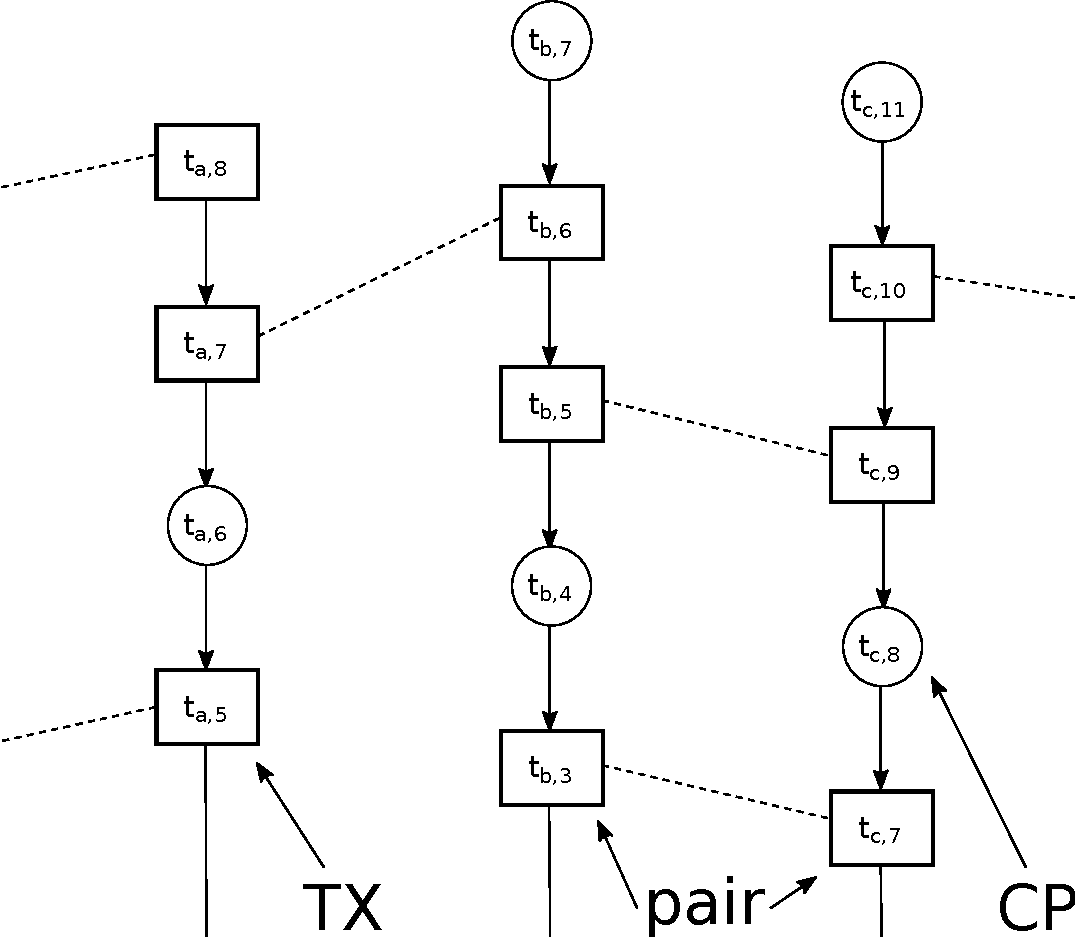
\includegraphics[width=\linewidth]{trustchain-good-cp}
\caption{Visualisation of the Extended TrustChain. $t_{u, i}$ represents a TX block on $u$'s chain with a sequence number of $i$.
$c_{v, j}$ represents a CP block on $v$'s chain with a sequence number of $j$.}
\label{fig:trustchain-good-cp}
\end{figure}

We randomly elect special nodes called facilitators in every round.
The facilitators reach consensus on CP blocks and the consensus result is essentially a set of CP blocks of from (nearly) all the nodes.
While this gives us consensus on a representation of the global state, it does not imply consensus on transactions.
To this end, we introduce the validation protocol that allows any nodes to challenge any other node to produce a set of TX blocks that computes to the CP block in consensus.
Hence we implicitly achieve consensus on transactions.

\subsection{Model and assumptions}
\label{sec:model-assumptions}

We assume purely asynchronous channels with eventual delivery.
Thus in no stage of our protocol do we make timing assumptions.
The adversary has full control of the delivery schedule and the message ordering of all messages.
But they are not allowed to drop messages except for their own\footnote{
    Reliability can be achieved in unreliable networks by resending messages or using some error correction code.
}.
Further, we assume there exists a Public Key Infrastructure (PKI),
and nodes are identified by their unique and permanent public key.

% TODO big N does not follow our convention
In our model, we consider $N$ nodes, which is the population size.
$n$ of them are facilitators, $t$ out of $n$ are malicious and the inequality
$n \ge 3t + 1$ must hold.
This is from the work of Pease, Shostak and Lamport, where they show a network of $n$ nodes cannot reach Byzantine agreement with $t \ge n/3$~\cite{pease1980reaching}.
Further, the inequality $N \ge n + t$ must also hold.
This is due to our system design, which becomes clear in~\Cref{sec:consensus-phase}.

Our threat model is as follows. 
We use a restricted version of the adaptive corruption model.
The first restriction is that corrupted node can only change across rounds.
That is, if a round has started, the corrupted nodes cannot change until the next round.
The second restriction is that the adversary, presumably controlling all the corrupted nodes, is forgetful.
Namely, the adversary may learn the internal state such as the private key of a corrupted node,
but if the node recovers, then the adversary must forget the private key.
This is realistic because otherwise the adversary can eventually learn all the private keys and sabotage the system.

\subsection{Extended TrustChain}
The primary data structure used in our system is the Extended TrustChain.
Each node $u$ has a public and private key pair---$pk_u$ and $sk_u$, and a chain $B_u$.
The chain consist of blocks $B_u = \{ b_{u, i} : i \in \{ 0, \dots, h - 1 \} \}$,
where $b_{u, i}$ is the $i$th block of $u$,
and $h$ is the height of the block (i.e. $h = |B_u|$).
We often use $b_{u, h}$ to denote the latest block.
There are two types of blocks, TX blocks and CP blocks.
If $T_u$ is the set of all TX blocks in $B_u$ and $C_u$ is the set of all CP blocks is $B_u$,
then it must be the case that $T_u \cup C_u = B_u$ and $T_u \cap C_u = \varnothing$.
The notation $b_{u, i}$ is generic over the block type.
We assume there exists a function $\textsf{typeof}: B_u \rightarrow \{ \tau, \gamma \}$ that returns the type of the block,
where $\tau$ represents the TX type and $\gamma$ represents the CP type.

\begin{definition}
\textbf{\emph{Transaction block}}

The TX block is a six-tuple, i.e
$$t_{u, i} = \langle \textsf{H}(b_{u, i - 1}), seq_u, txid, pk_v, m, sig_u \rangle.$$
We describe each item in turn.
\begin{enumerate}
\item $\textsf{H}(b_{u, i - 1})$ is the hash pointer to the previous block.
\item $seq_u$ is the sequence number which should equal $i$.
\item $txid$ is the transaction identifier, it should be generated using a cryptographically secure pseudo-random number generator by the initiator of the transaction.
\item $pk_v$ is the public key of the counterparty $v$.
\item $m$ is the transaction message.
\item $sig_u$ is the signature created using $sk_u$ on the concatenation of the binary representation of the five items above.
\end{enumerate}
The fact that we have no constraint on the content of $m$ is in alignment with our design goal---application neutrality.

TX blocks come in pairs.
In particular, for every block 
$$t_{u, i} = \langle \textsf{H}(b_{u, i - 1}), seq_u, txid, pk_v, m, sig_u \rangle$$
there exist one and only one \emph{pair} 
$$t_{v, j} = \langle \textsf{H}(b_{v, j - 1}), seq_v, txid, pk_u, m, sig_v \rangle.$$
Note that the $txid$ and $m$ are the same, and the public keys refer to each other.
Thus, given a TX block, these properties allow us to identify its pair.
\end{definition}

% TODO Node $v$ may cheat and create more than one pair for $t_{u, i}. we discuss later

\begin{definition}
\textbf{\emph{Checkpoint block}}

The CP block is a five-tuple, i.e. 
$$c_{u, i} = \langle \textsf{H}(b_{u, i-1}), seq_u, \textsf{H}(\C_r), r, sig_u \rangle,$$
where $\C_r$ is the consensus result (which we describe in \Cref{sec:consensus-result}) in round $r$,
the other items are the same as the TX block definition.
% Note that unlike in our prior work~\cite{implicitconsensus}, CP blocks and TX blocks do not have independent sequence numbers.

The genesis block in the chain must be a CP block in the form of
$$c_{u, 0} = \langle \textsf{H}(\bot), 0,  \textsf{H}(\bot), 0, sig_u \rangle,$$
where $\textsf{H}(\bot)$ can be interpreted as applying the hash function on an empty string.
The genesis block is unique because every node has a unique public and private key pair.
\end{definition}


\begin{definition}
\label{sec:consensus-result}
\textbf{\emph{Consensus result}}

Our consensus protocol runs in rounds.
Every round is identified by a round number $r$, which is incremented on every new round.
The consensus result is a tuple, i.e. $\C_r = \langle r, C \rangle$,
where $C$ is a set of CP blocks agreed by the facilitators of round $r$.
\end{definition}

Here we define an important property which results from the interleaving nature of CP and TX blocks.
It is used in our validation protocol.
\begin{definition}
\textbf{\emph{Enclosure and agreed enclosure}}

If there exist a tuple $\langle c_{u,a}, c_{u, b} \rangle$ for a TX block $t_{u, i}$,
where 
$$a = \argmin_{k, k < i, \texttt{typeof}(b_{u,k}) = \gamma}(i - k)$$
$$b = \argmin_{k, k > i, \texttt{typeof}(b_{u,k}) = \gamma}(k - i),$$
then $\langle c_{u,a}, c_{u, b} \rangle$ is the enclosure of $t_{u, i}$.
Intuitively, that is the two closest CP blocks that surround $t_{u, i}$.
Note that $c_{u, a}$ is the more recent CP block.
Also, some TX blocks may not have any enclosure, then its enclosure is $\bot$.
Agreed enclosure is the same as enclosure with an extra constraint where the CP blocks must be in some consensus result $\C_r$.
\end{definition}


\begin{definition}
\textbf{\emph{Fragment and agreed fragment}}

If the enclosure of some TX block $t_{u, i}$ is $\langle c_{u,a}, c_{u, b} \rangle$,
then its \emph{fragment} $F_{u, i}$ is defined as $\{ b_{u, i} : a \le i \le b \}$.
Similarly, \emph{agreed fragment} has the same definition as fragment but using agreed enclosure.
For convenience, the function $\textsf{agreed\_fragment}(\cdot)$ represents the agreed fragment of some TX block if it exists, otherwise $\bot$.
\end{definition}

\subsection{Consensus Protocol}
Our scalable consensus protocol runs on top of Extended TrustChain.
It uses an unmodified asynchronous subset consensus (ACS) algorithm as the key building block.
The objectives of the protocol are to
    allow honest nodes always make progress (in the form of creating new CP blocks),
    compute correct consensus result in every round
    and have an unbiased election of facilitators.
Concretely, we define the necessary properties as follows.
\begin{definition}
\label{def:consensus}
\textbf{\emph{Properties of the consensus protocol}}

$\forall r \in \mathbb{N}$, the following properties must hold.
\begin{enumerate}
    \item \emph{Agreement}:
        If one correct node outputs a set of facilitators $\F_r$,
        then every node outputs $\F_r$
    \item \emph{Validity}:
        If any correct node outputs $\F_r$, then 
            \begin{enumerate}
                \item $|\C_r| \ge N - t$ and each CP in $\C_r$ belong to a different node\footnote{
                $\C_r$ is a tuple but we abuse the notation here by writing $|\C_r|$ to mean the number of CP blocks in the second element of $\C_r$.}.
                \item $\F_r$ must contain at least $n - t$ honest nodes and
                \item $|\F_r| = n$.
            \end{enumerate}
    \item \emph{Fairness}:
        Every node with a CP block in $\C_r$ should have an equal probability of becoming a member of $\F_r$.
    \item \emph{Termination}:
        Every correct node eventually outputs some $\F_r$.
\end{enumerate}
\end{definition}
These properties are similar to Byzantine consensus properties but there are subtle differences.
Firstly, they are properties for every node in the network and not just the facilitators.
Secondly, they must be satisfied for all rounds because the whole system falls apart if one of the property cannot be satisfied in one of the rounds.


\subsubsection{Bootstrap phase}
\label{sec:bootstrap}
As with many distributed systems, there must be a bootstrap phase which sets up the system.
Imagine that there is some bootstrap oracle, that initiates the code on every node.
The code satisfies all the properties in \Cref{def:consensus}.
Namely, every node has the same set of valid facilitators $\F_1$ that are randomly chosen.
This concludes the bootstrap phase.
For any future rounds, the consensus phase is used.

In practice, the bootstrap oracle is most likely the software developer and some of the desired properties cannot be achieved.
In particular, it is not possible to have the fairness property because it is unlikely that the developer knows the identity of every node in advance.

\subsubsection{Consensus phase}
\label{sec:consensus-phase}
The consensus phase begins when $\F_r$ is available to all the nodes.
Note that $\F_r$ indicates the facilitators that were elected using results of round $r$ and are responsible for driving the ACS protocol in round $r + 1$.
The goal is to reach agreement on a set of new facilitators $\F_{r + 1}$ that satisfies the four properties in \Cref{def:consensus}.

There are two scenarios in the consensus phase.
First, if node $u$ is not the facilitator, it sends $\langle \texttt{cp\_msg}, c_{u, h} \rangle$ to all the facilitators.
Second, if the node is a facilitator, it waits until $N - t$ messages of type \texttt{cp\_msg} are received.
% Second if the node is a facilitator, it waits for some duration $D$ and collect messages of type \texttt{cp\_msg}, where $D \gg \Delta$.
Invalid messages are removed.
That is blocks with invalid signatures and blocks signed by the same key.
With the sufficient number of \texttt{cp\_msg} messages,
it begins the ACS algorithm and some $\C'_{r + 1}$ should be agreed upon by the end of it.
Duplicates and blocks with invalid signatures are again removed from $\C'_{r+1}$ and we call the final result $\C_{r+1}$.
We have to remove invalid blocks a second time (after ACS) because the adversary may send different CP blocks to different facilitators,
which results in invalid blocks in the ACS output, but not in any of the inputs.

The core of the consensus phase is the ACS protocol.
While any ACS protocol that satisfies the standard definition will work,
we use a simplification of HoneyBadgerBFT~\cite{miller2016honey} as our ACS protocol
because it is a consensus algorithm designed for blockchain systems.
We do not use the full HoneyBadgerBFT due to the following.
First, the transactions in HoneyBadgerBFT are first queued in a buffer and the main consensus algorithm starts only when the buffer reaches an optimal size.
We do not have an infinite stream of CP blocks, thus buffering is unsuitable.
Second, HoneyBadgerBFT uses threshold encryption to hide the content of the transactions.
But we do not reach consensus on transactions, only CP blocks, so hiding CP blocks is meaningless for us as it contains no transaction information.

Continuing, when $\F_{r}$ reaches agreement on $\C_{r+1}$,
they immediately broadcast\footnote{An alternative to using broadcasting is to use an epidemic protocl~\cite{eugster2004epidemic}, 
as long as it can guarantee delivery.} two messages to all the nodes---
first the consensus message $\langle \texttt{cons\_msg}, \C_{r+1} \rangle$,
and second the signature message $\langle \texttt{cons\_sig}, r, sig \rangle$.
The reason for sending \texttt{cons\_sig} is the following.
Recall that channels are not authenticated, 
and there are no signatures in $\C_{r + 1}$.
If a non-facilitator sees some $\C_{r + 1}$, it cannot immediately trust it because it may have been forged.
Thus, To guarantee authenticity, every facilitator sends an additional message that is the signature of $\C_{r + 1}$.

Upon receiving $\C_{r + 1}$ and at least $n - f$ valid signatures by some node $u$, $u$ performs two tasks.
First, it creates a new CP block using $\textsf{new\_cp}(\C_{r + 1}, r + 1)$ using \Cref{alg:new-cp}.
Second, it computes the new facilitators using $\textsf{get\_facilitator}(\C_{r + 1}, n)$ using \Cref{alg:facilitator},
and updates its facilitator set to the result.
This concludes the consensus phase and brings us back to the beginning of the consensus phase.

\begin{algorithm}
\caption{Function $\textsf{new\_cp}(\C_r, r)$ runs in the context of the caller $u$.
It creates a new CP block and appends it to $u$'s chain.}
\label{alg:new-cp}
\begin{algorithmic}
\State $h \gets |B_u|$
\State $c_{u, h} \gets \langle \textsf{H}(b_{u, h-1}), h, \textsf{H}(\C_r), r, sig_u \rangle$
\State $B_u \gets B_u \cup c_{u, h}$
\end{algorithmic}
\end{algorithm}

\begin{algorithm}
\caption{Function $\textsf{get\_facilitator}(\C_r, n)$ takes the consensus result $\C_r$ and an integer $n$,
then sorts the CP blocks $C$ by the luck value (the $\lambda$-expression), and outputs the smallest $n$ elements.}
\label{alg:facilitator}
\begin{algorithmic}
\State $\langle r, C \rangle \gets \C_r$
\State $\textsf{take} (n, \textsf{sort\_by} (\lambda x.\textsf{H}(\C_r || pk \text{ of } x), C))$
\end{algorithmic}
\end{algorithm}


Our protocol has some similarities with synchronizers~\cite[Chapter 10]{podc} because it is effectively a technique to introduce synchrony in an asynchronous environment.
If we consider the facilitators as a collective authority, then it can be seen as a synchronizer that sends pulse messages (in the form of \texttt{cons\_msg} and \texttt{cons\_sig}) to indicate the start of a new clock pulse.
Every node then sends a completion messages (in the form of \texttt{cp\_msg}) to the new collective authority to indicate that they are ready for the next pulse.

\subsection{Transaction Protocol}
\label{sec:tx-protocol}

The TX protocol, shown in \Cref{alg:tx-proto}, is run by all nodes.
It is also known as True Halves, first described by Veldhuisen~\cite[Chapter~3.2]{truehalves}.
Nodes that wish to initiate a transaction calls $\textsf{new\_tx}(pk_v, m, txid)$ (\Cref{alg:new-tx}) with the intended counterparty $v$ identified by $pk_v$ and message $m$.
$txid$ should be a uniformly distributed random value, i.e. $txid \in_R \{0, 1\}^{256}$.
Then the initiator sends $\langle \texttt{tx\_req}, t_{u, h}\rangle$ to $v$.

\begin{algorithm}
    \caption{Function $\textsf{new\_tx}(pk_v, m, txid)$ generates a new TX block and appends it to the caller $u$'s chain.
    It is executed in the private context of $u$, i.e. it has access to the $sk_u$ and $B_u$.
    The necessary arguments are the public key of the counterparty $pk_v$, the transaction message $m$ and the transaction identifier $txid$.}
    \label{alg:new-tx}

    \begin{algorithmic}
    \State $h \gets |B_u|$
    \State $t_{u, h} \gets \langle \textsf{H}(b_{u, h - 1}), h, txid, pk_v, m, sig_u \rangle$
    \State $B_u \gets B_u \cup \{ t_{u, h} \}$
    \end{algorithmic}
\end{algorithm}

\begin{algorithm}
    \caption{The TX protocol which runs in the context of node $u$.}
    \label{alg:tx-proto}

    \begin{algorithmic}
        \Upon $\langle \texttt{tx\_req}, t_{v, j} \rangle$ from $v$
        \State $\langle \_, \_, txid, pk_v, m, \_ \rangle \gets t_{v, j}$
        \State $\textsf{new\_tx}(pk_u, m, txid)$
        \State store $t_{v, j}$ as the pair of $t_{u, h}$
        \State send $\langle \texttt{tx\_resp}, t_{u, h} \rangle$ to $v$

        \Upon $\langle \texttt{tx\_resp}, t_{v, j} \rangle$ from $v$
        \State $\langle \_, \_, txid, pk_v, m, \_ \rangle \gets t_{v, j}$
        \State store $t_{v, j}$ as the pair of the TX with identifier $txid$
    \end{algorithmic}
\end{algorithm}

A key feature of the TX protocol is that it is non-blocking.
At no time in \Cref{alg:new-tx} or \Cref{alg:tx-proto} do we need to hold the chain state and wait for some message to be delivered before committing a new block to the chain.
This allows for high concurrency where we can call $\textsf{new\_tx}(\cdot)$ multiple times without waiting for the corresponding \texttt{tx\_resp} messages.

\subsection{Validation protocol}
\label{sec:vd-protocol}

Up to this point, we do not provide a mechanism to detect tampering.
The validation protocol aims to solve this issue.
The protocol is also a request-response protocol, just like the transaction protocol.
But before explaining the protocol itself, we first define what it means for a transaction to be valid.

\subsubsection{Validity definition}
A transaction can be in one of three states in terms of validity---\emph{valid}, \emph{invalid} and \emph{unknown}.
Given a fragment $F_{v, j}$, the validity of the TX block $t_{u, i}$ and the agreed fragment of it is captured by the function $\textsf{get\_validity}(t_{u, i}, F_{u, i}, F_{v, j})$ (\Cref{alg:get-validity}).
Note that $t_{u, i}$ and $F_{u, i}$ are assumed to be valid,
otherwise the node calling the function would have no point of reference.
This is not difficult to achieve.
Typically the caller is $u$, so it knows its own TX block and the corresponding agreed fragment.
If the caller is not $u$, it can always query for the agreed fragment that contains the transaction of interest from $u$.

\Cref{alg:get-validity} works as follows.
Before~\Cref{line:valid-fragment},
we essentially check whether the fragment is the one that the verifier needs.
If it is not, then the verifier cannot make any decision and return \emph{unknown}.
This is likely to be the case for new transactions because the result of $\textsf{agreed\_fragment}(\cdot)$ would be $\bot$.
The next two conditions check for tampering or missing blocks, if any of these misconducts are detected, then the TX is invalid.

We stress that the \emph{unknown} state means that the verifier does not have enough information to continue with the validation protocol.
If enough information is available at a later time, then the verifier will output either \emph{valid} or \emph{invalid}.

Note that the validity is on a transaction (two TX blocks with the same $txid$), rather than on one TX block owned by a single party.
It is defined this way because the malicious sender may create new TX blocks in their own chain but never send \texttt{tx\_req} messages.
In that case, it may seem that the counterparty, who is honest, purposefully omitted TX blocks.
But in reality, it was the malicious sender who did not follow the protocol.
Thus, in such cases, the whole transaction identified by its $txid$ is marked as invalid.

Further, the caller of $\textsf{get\_validity}(t_{u, i}, F_{u, i}, F_{v, j})$ is not necessarily 
$u$\footnote{In practice, it often is because after completing the TX protocol the parties are incentivised to check that the counterparty ``did the right thing''.}
Any node $w$ may call $\textsf{get\_validity}(t_u{u, i}, F_{u, i}, F_{v, j})$ as long as $w$ has an the necessary input parameters.
$F_{u, i}$  and $t_{u, i}$ may be readily available if $w = u$.
Otherwise, $w$ could query $u$ with the \texttt{vd\_req} message and then obtain the result from \texttt{vd\_resp}.
This is the validation protocol which we describe next.

\begin{algorithm}
\caption{Function $\textsf{get\_validity}(t_{u, i}, F_{u, i}, F_{v, j})$ validates the transaction represented by $t_{u, i}$.
We assume $F_{u, i}$ is always correct and contains $t_{u, i}$.
$F_{v, j}$ is the corresponding fragment received from $v$.}
\label{alg:get-validity}

\begin{algorithmic}

    \If{$F_{v, j}$ is not a fragment created in the same round as $F_{u, i}$}
        \State \Return \emph{unknown}
    \EndIf

    \label{line:valid-fragment}
    \State $\langle \_, \_, txid, pk_v, m, \_ \rangle \gets t_{u, i}$
    \If{number of blocks of $txid$ in $F_{v, j} \ne 1$}
        \State \Return \emph{invalid}
    \EndIf

    \State $t_{v, j} \gets $ the TX block with $txid$ in $F_{v, j}$
    \State $\langle \_, \_, txid', pk_u, m', \_ \rangle \gets t_{v, j}$ 

    % message tampering
    \If{$m \ne m' \vee txid \ne txid'$} 
        \State \Return \emph{invalid}
    \EndIf

    % signature tampering
    \If{$t_{u, i} \text{ is not signed by } pk_u \vee t_{v, j} \text{ is not signed by } pk_v $}
        \State \Return \emph{invalid}
    \EndIf
    \State \Return \emph{valid}
\end{algorithmic}
\end{algorithm}

\subsubsection{Validation protocol}
Our validation protocol,
shown in~\Cref{alg:vd-proto},
is designed to classify transactions according to the aforementioned validity definition.
If $u$ wishes to validate some TX with ID $txid$ and counterparty $v$, it sends $\langle \texttt{vd\_req}, txid \rangle$ to $v$.
The desired properties of the validation protocol are as follows.
\begin{definition}
\label{def:validation}
\textbf{\emph{Properties of the validation protocol}}

\begin{enumerate}
    \item \emph{Agreement}:
        If any correct node decides on the validity (except when it is \emph{unknown}) of a transaction,
        then all other correct nodes are able to reach the same conclusion or \emph{unknown}.
    \item \emph{Validity}:
        The validation protocol outputs the correct result
        according to the aforementioned validity definition.
    % \item \emph{Unforgeability}:
    %     If some transaction is valid, it cannot be forged into an invalid transaction.
    %     If some transaction is invalid, it cannot be forged into a valid transaction.
    \item \emph{Liveness}:
        Any valid (invalid) transaction is marked as valid (invalid) eventually.
\end{enumerate}
\end{definition}

\begin{algorithm}
\caption{Validation protocol which runs in the context of $u$}
\label{alg:vd-proto}

\begin{algorithmic}
    \Upon $\langle \texttt{vd\_req}, txid \rangle$ from $v$
        \State $t_{u, i} \gets \text{the transaction identified by } txid$
        \State $F_{u, i} \gets \textsf{agreed\_fragment}(t_{u, i})$
        \State send $\langle \texttt{vd\_resp}, txid, F_{u, i} \rangle$ to $v$

    \Upon $\langle \texttt{vd\_resp}, txid, F_{v, j} \rangle$ from $v$
        \State $t_{u, i} \gets \text{the transaction identified by } txid$
        \If{$F_{u, i}$ and $F_{v, j}$ are available and $F_{u, i}$ is the agreed fragment of $t_{u, i}$}
            \State set the validity of $t_{u, i}$ to $\textsf{get\_validity}(t_{u, i}, F_{u, j}, F_{v, j})$
        \EndIf
\end{algorithmic}
\end{algorithm}

We make two remarks.
First, just like the TX protocol, we do not block at any part of the protocol.
Second, suppose some $F_{v, j}$ validates $t_{u, i}$, then that does not imply that $t_{u, i}$ only has one pair $t_{v, j}$.
Our validity requirement only requires that there is only one $t_{v, j}$ in the correct consensus round.
The counterparty may create any number of fake pairs in later consensus rounds.
But these fake pairs only pollutes the chain of $v$ and can never be validated because the round is incorrect.

\subsection{Design variations and tradeoffs}
\label{sec:tradeoffs}

Up to this point,
we have discussed our protocol in the context of the model and assumptions defined in \Cref{sec:model-assumptions}.
In this section, 
we explore a few design variations which we can make, some of them require a relaxed version of our original model.
They enable better performance, allow us to apply our design in the fully permissionless setting and improves privacy.

\subsubsection{Using timing assumption in the permissionless setting}
\label{sec:permissionless}
Our model is purely asynchronous, where we make no timing assumptions anywhere in the protocol.
However, in many applications it is often fine to make timing assumptions.
For example, TCP relies on timeout for its retransmission and the \texttt{nLockTime} property in Bitcoin transactions makes the transaction unspendable until some time in the future (either Unix time or block height)~\cite{bitcoindevguide}.
One limitation of our system is that we use the parameter $N$ in our algorithms, which makes it unsuitable for the permissionless environment where users can join and leave at will.
In this section we show how making a timing assumption would allow us to operate in the permissionless setting.

At the start of our consensus phase (\Cref{sec:consensus-phase}), facilitators must wait for $N-f$ \texttt{cp\_msg} messages.
This is the only place where we used $N$ as a parameter.
To introduce timing, instead of waiting for $N-f$ messages, we wait for some time $D$,
such that $D$ is sufficiently long for honest nodes to send their CP blocks to the facilitators.
Consequently, this removes the need for a PKI because the collected CP blocks may be from nodes that nobody has seen in the past.
However, choosing the parameter $D$ is difficult and depends on a number of factors such as the network condition, message size, and so on.
Overestimating it would make agreed fragments much longer than usual, which increases communication costs for validation.
Underestimating it would lead to unfairness where users with a poor internet connection will have a lower chance to be selected as a facilitator in the next round.
Nevertheless, there is a significant gain for making the timing assumption and that is the ability to operate in the permissionless setting which we explain next.

Suppose a new node wish to join the network and the facilitators are known (this can be done with a public registry).
It simply sends its latest CP block to the facilitators.
Then, in the next round, the node will have a chance to become a facilitator just like any existing node.
To leave the network, nodes simply stop submitting CP blocks.
There is a subtlety here which happens when the node is elected as a facilitator in the following round.
In this case, the node must fulfil its obligation by completing the consensus protocol, but without proposing its own CP block, before leaving.
Otherwise, the $n \ge 3t + 1$ condition may be violated.

\subsubsection{Privacy preserving validation protocol using compact blocks}
\label{sec:compact}
Our approach already has privacy preserving features in comparison to early blockchain systems.
That is, the transactions for each node are only revealed during the validation protocol.
Hence if two nodes never directly or indirectly interact with each other,
their transactions are never revealed.

We can take our privacy-preserving property one step further by introducing another level of hash pointer indirection.
The result is shown in~\Cref{fig:compact}.
\begin{figure}
    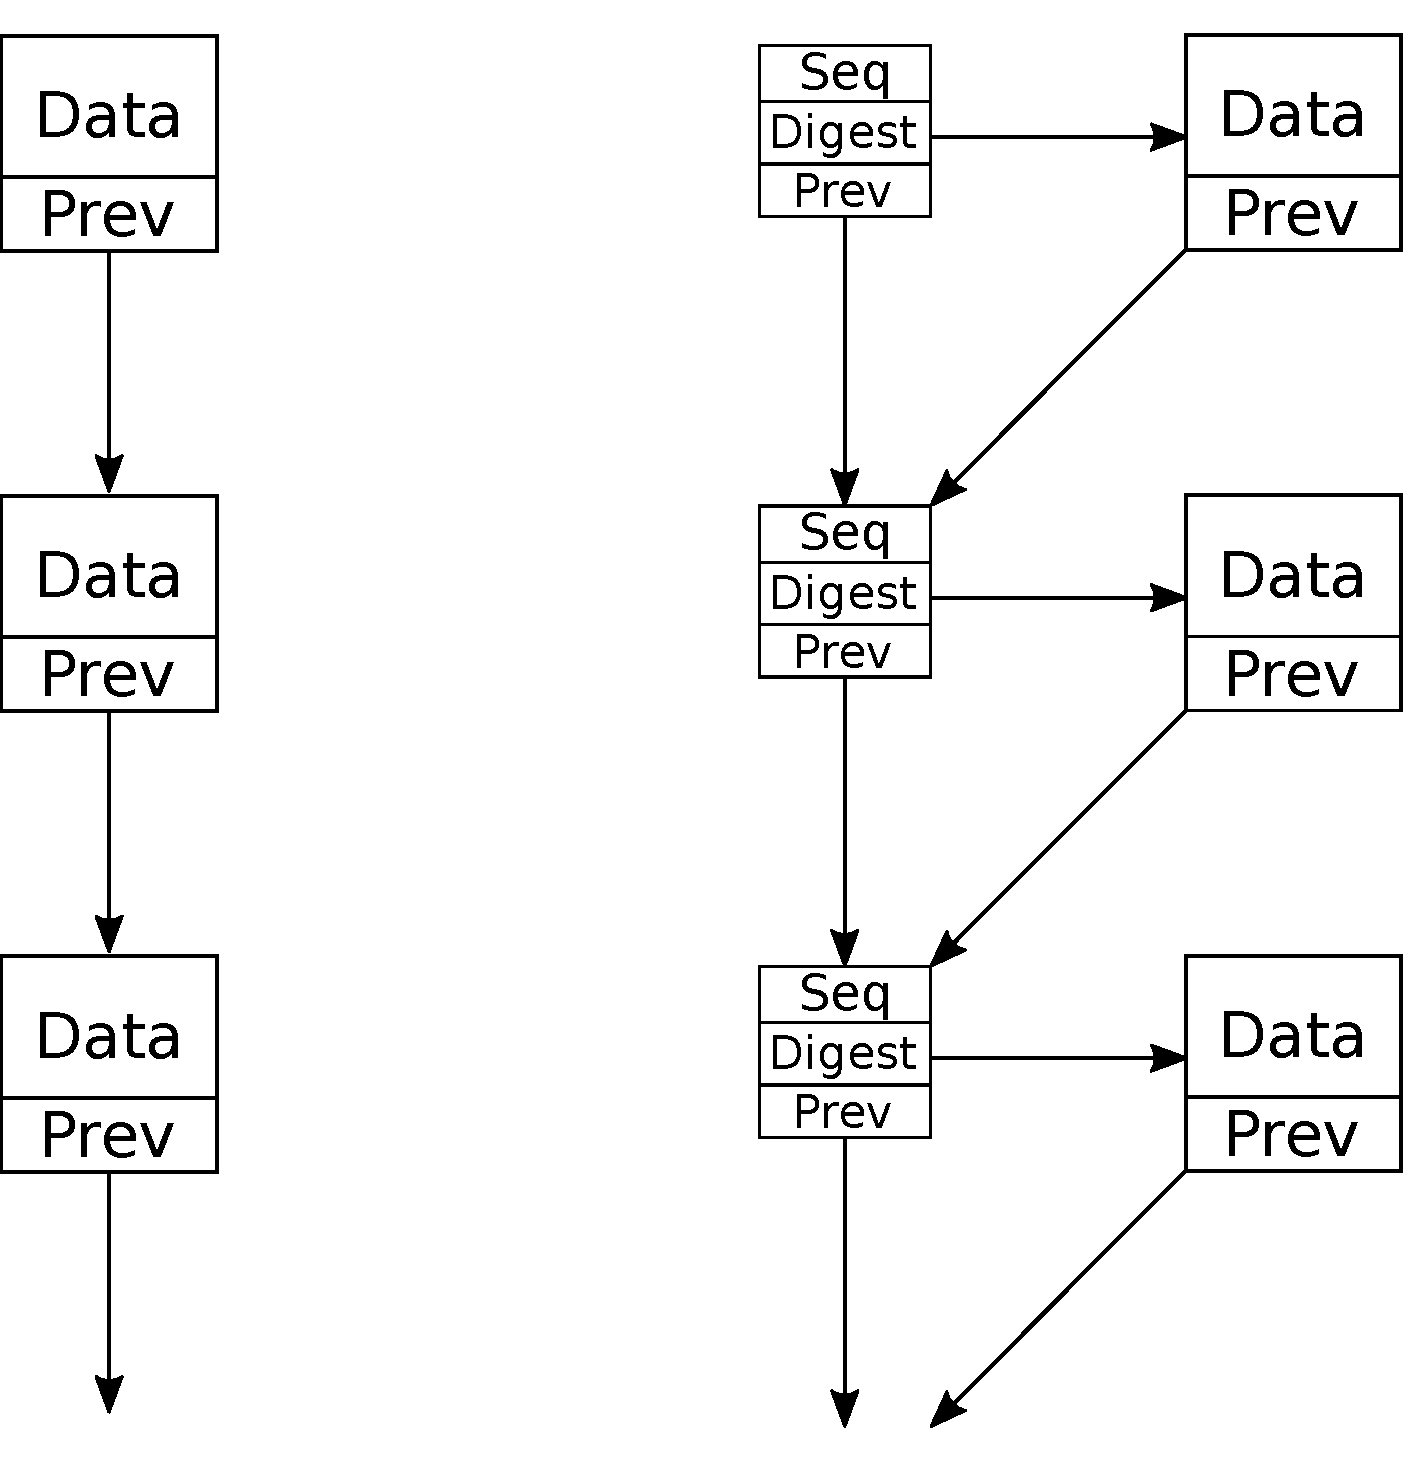
\includegraphics[width=0.7\linewidth]{compact}
    \centering
    \caption{The chain on the left represent direct chaining, where the digest in ``Prev'' is simply the digest of the previous block.
    The chain on the right uses compact blocks, represented by the smaller squares.
    Compact blocks also form a chain as before, but they each have a hash pointer to the full block, identified by ``Seq'' and ``Digest''.}
    \label{fig:compact}
\end{figure}

Concretely, we introduce an additional block type,
namely compact block.
Such blocks only have three attributes,
\begin{enumerate}
\item Seq---the sequence number its corresponding block,
\item Digest---the digest of its corresponding block, and
\item Prev---the digest of the previous compact block.
\end{enumerate}
Each compact block has a corresponding full block (either a CP block or a TX block).
The relationship is uniquely identified with Seq or Digest.
Recall that our original validation protocol requires the nodes to send the full agreed fragment.
With compact blocks, it is only necessary to send the compact version of the agreed fragment.
The validation then proceeds in a similar fashion,
provided that the pair of the to-be-validated TX block is known.

\subsubsection{Optimising validation protocol using cached agreed fragments}
\label{sec:caching}
One more way to improve the efficiency of the validation protocol is to use a single agreed fragment to validate multiple transactions.
Concretely, upon receiving an agreed fragment from node $A$,
rather than validating a single transaction,
we attempt to validate all transactions with $A$ in the unknown state in that fragment.

For a node, the benefit of this technique is maximised when it only transacts with one other node.
In this case, the communication of one fragment is sufficient to validate all transactions in that fragment.
In the opposite extreme, if every transaction that the node makes is with another unique node,
then the caching mechanism would have no effect.

\subsubsection{Global fork detection}
The validation algorithm guarantees that there are no forks within a single agreed fragment.
This is sufficient for some applications such as proving the existence of some information.
However, for applications such as digital cash where every block depends on one or more previous blocks,
our scheme is not suitable.
For such applications, we need to guarantee that there are no forks from the genesis block leading up to the TX block of interest.

There are a variety of approaches to do global fork detection.
First and the easiest solution is to simply ask for the complete chain of the counterparty.
The verifier can be sure that there are no forks if the following holds.
\begin{enumerate}
    \item The hash pointers are correct.
    \item All the CP blocks are in consensus.
    \item The TX of interest is in the chian.
\end{enumerate}
We use this approach in our prior work on Implicit Consensus~\cite{implicitconsensus}.
It may sound inefficient at first, but nodes employ caching to minimise communication costs.

The second approach is probabilistic but with only a constant communication overhead over our current design.
For a node, observe that if all of its agreed fragments has a transaction with an honest node,
then the complete chain is effectively validated in a distributed manner.
The only way for an attacker to make a fork is to make sure that the agreed fragment containing the fork has no transactions with honest nodes.
Such malicious behaviour is prevented probabilistically using a challenge-response protocol as follows.
Suppose node $A$ wish to make a transaction with node $B$.
$A$ first sends a challenge to $B$ asking it to prove that it holds a valid agreed fragment between some consensus round specified by $A$.
If $B$ provides a correct proof, then they run the transaction protocol as usual.
If $B$ provides an invalid proof or refuses to respond,
then $A$ would refuse to make the transaction.


\section{Correctness and fault tolerance analysis}
\label{sec:analysis}
Here we evaluate our system analytically to ensure the desired properties (\Cref{def:consensus} and \Cref{def:validation}) hold.
An informal argument is given in this section, we refer to~\cite{checo}??? for an indepth analysis.

\subsection{Correctness of the consensus protocol}
Recall that the consensus protocol properties (\Cref{def:consensus}) has
four conditions---agreement, validity, fairness and termination.
Agreement, validity and termination hold due to the fact that the following three facts
\begin{enumerate}
    \item The CP blocks sent to the facilitators are eventually delivered and then ACS eventually starts.
    \item Agreement, validity and termination holds for ACS.
    \item The consensus result and signatures are eventually disseminated to all the nodes.
\end{enumerate}

Fairnress holds if we model $\textsf{H}(\cdot)$ as a query to the random oracle.
Sorting nodes by the luck value $\textsf{H}(\C || pk)$ can be seen as a random permutation of a list of nodes.
Therefore every node has the same probability of becoming a facilitator.

\subsection{Correctness of the validation protocol}
Using the previous result,
we show that the agreement and validity properties (from~\Cref{def:validation}) hold for the validation protocol.

The validty property holds because we use $\textsf{get\_validity}(\cdot)$ in the validation protocol.
The agreement property holds due to the collision resistent property of cryptographically secure hash function.
Suppose two honest nodes decided on two different state, \emph{valid} and \emph{invalid} for the same transaction.
Due to the properties of the consensus protocol, the agreed enclosure for the transaction must be the same.
For that to happen, two agreed fragments must exist for the same transaction.
Recall that blocks form a hash chain.
So this cannot happen unless the hash function is not cryptographically secure.

Liveness, unfortunately does not hold in our model.
A malicious node can ask honestly when running the transaction protocol,
but then never respond to any validation requests.
Therefore there are transactions that can never be validated.
Nevertheless, the malicious node will be at an economical loss if it is not responsive because honest nodes are less likely to make contact with nodes that do not respond to validation messages.

A stronger version of the validity definition exists.
That is, if two honest nodes make a transaction,
then the transaction state is always valid in addition to our current validity definition.
Under our purely asynchronous model, we cannot guarantee this stronger version.
Since the adversary can delay any message for any amount of time,
it can make sure all \texttt{tx\_req} messages are delivered in a round later than the round which the message is sent.
Effectively, the transaction pair would always be in different rounds and the validation protocol would not output \emph{valid}.
We believe in a relaxed model, i.e. a weakly synchronous model, a stronger validity definition is possible.

\subsection{Fault tolerance}
Finally, we consider the effect when the number of adversaries is more than $t$.
This is useful because in practice it is difficult to guarantee that $t$ satisfies $n \ge 3t + 1$,
especially when $N$ is large.
Hence we are interested in the probability for this to happen under our facilitator election process.
The problem is modeled by a hypergeometric distribution,
where the random variable $X$ is the number of malicious nodes.
For our system to fail, we are interested in the following probability.
$$
\Pr[X \ge \lfloor \frac{n-1}{3} \rfloor + 1]
$$
Let $E[X] = n\alpha$ where $0 \le \alpha \le \lfloor \frac{n-1}{3} \rfloor/n < (\lfloor  \frac{n - 1}{3} \rfloor + 1) / n$.
Using the tail inequality found in~\cite{skala2013hypergeometric}
$$
\Pr[X \ge E[X] + \tau n] \le e^{-2\tau^2n},
$$
and setting 
$$
\tau = \frac{\lfloor \frac{n-1}{3} \rfloor + 1}{n} - \alpha,
$$
we arrive at the following bound
$$
\Pr[X \ge \lfloor \frac{n-1}{3} \rfloor + 1] \le e^{-2 \big(\frac{\lfloor  \frac{n - 1}{3} \rfloor + 1}{n} - \alpha \big)^2 n}.
$$

The bound is not tight, but it is useful for picking parameters.
If $n$ is known, then we can pick a $\alpha$ such that the probability becomes small.
On the other hand, if $\alpha$ is fixed, but small, we may increase $n$ to achieve the same.
Furthermore, hypergeometric distributions have light tails with ``faster-than-exponential fall-off''~\cite{skala2013hypergeometric},
the probability for picking more than $\lfloor \frac{n-1}{3} \rfloor$ malicious nodes drops of exponentially as the expected value moves away from $\lfloor \frac{n-1}{3} \rfloor$.
To put this into perspective,
suppose $n = 1000$ and $\alpha = 1/5$, i.e. a fifth of the nodes are malicious.
Then the probability to draw more black balls than the threshold is only $2.6 \times 10^{-16}$.




\section{Implementation and Evaluation}
\label{sec:implementation}

\begin{figure*}[t]
  \centering
  \makebox[\linewidth][c]{%
  \begin{subfigure}[b]{0.5\linewidth}
    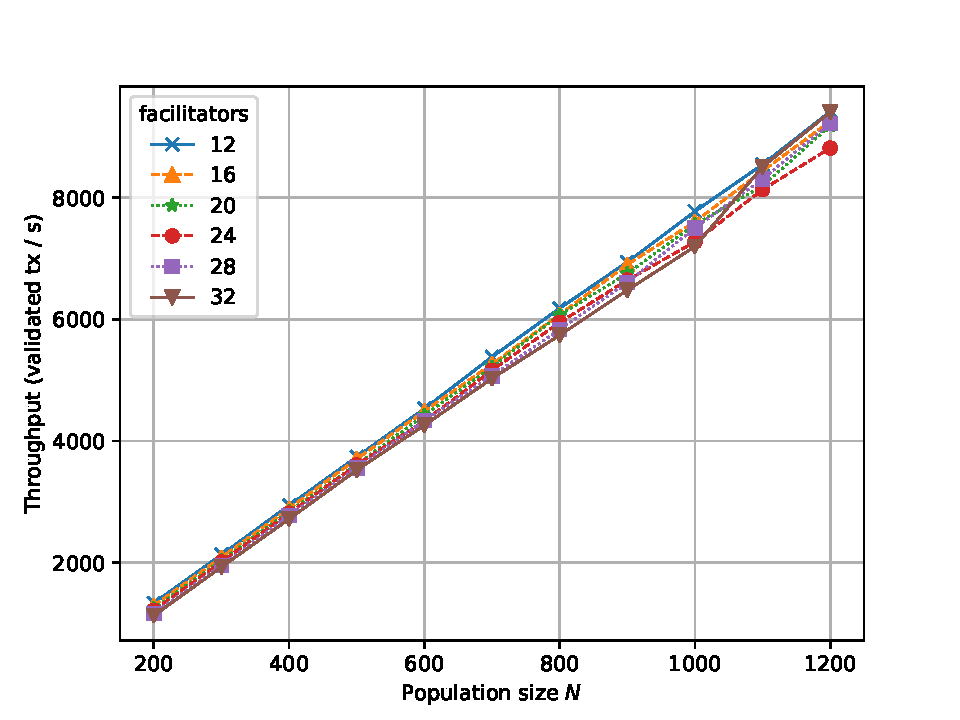
\includegraphics[width=\linewidth]{neighbour-fixed/throughput-vs-population}
    \caption{Every node make transactions with a fixed node.}
    \label{fig:global-throughput-fixed}
  \end{subfigure}%
  \begin{subfigure}[b]{0.5\linewidth}
    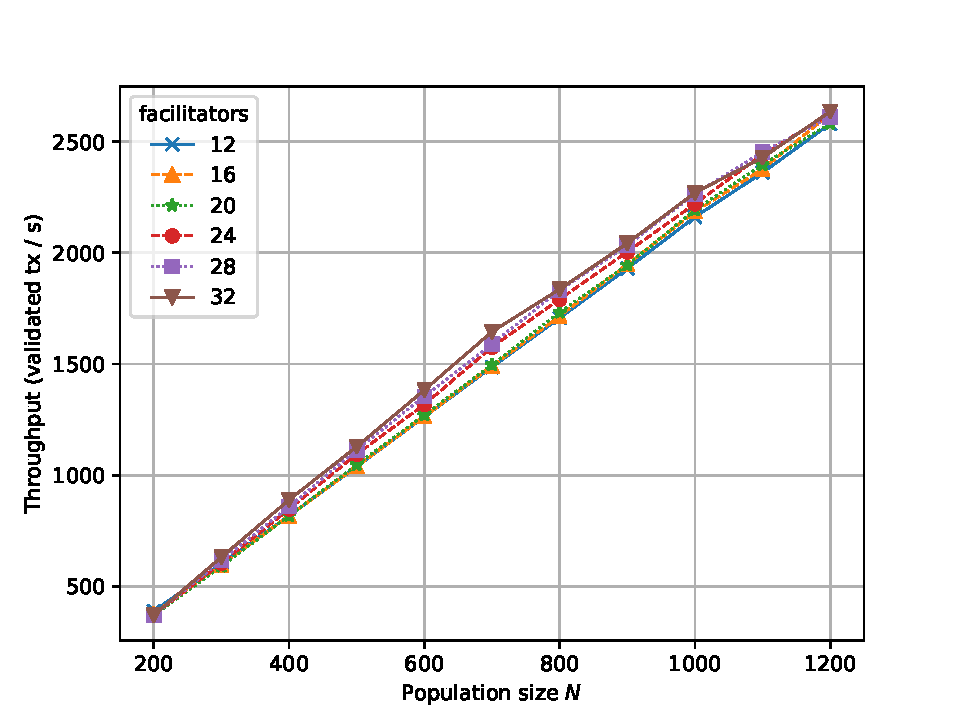
\includegraphics[width=\linewidth]{neighbour-random/throughput-vs-population}
    \caption{Every node make transactions with a random node.}
    \label{fig:global-throughput-random}
  \end{subfigure}
  }
  \caption{Global throughput increases as the population increases when every node transact at the same rate.
  Making transactions with fixed nodes results in a higher throughput because of the caching mechanism.}
  \label{fig:global-throughput}
\end{figure*}

The prototype implementation can be found on GitHub.
\begin{displayquote}
\url{https://github.com/kc1212/consensus-thesis-code}
\end{displayquote}
It implements the three protocols and the Extended TrustChain.
We also implement the caching optimisations discussed in \Cref{sec:caching}.
It is written in the Python programming language\footnote{\url{https://www.python.org/}}.
The cryptography primitives we use are SHA256 for hash functions and Ed25519 for digital signatures.
Both of which are provided by libnacl~\footnote{\url{https://pypi.python.org/pypi/libnacl}}.

We run the experiment on the DAS-5\footnote{\url{https://www.cs.vu.nl/das5/}} with up to 1200 nodes.
Every node makes transactions at 2 per second.
Since Bitcoin transactions are approximately 500 bytes~\cite{txsize},
we use a uniformly random transaction size sampled between 400 and 600 bytes.

To coordinate nodes on many different machines,
we employ a discovery server to inform every node the IP addresses and port numbers of every other node.
It is only run before the experiment and is not used during the experiment.

The global throughput results are shown in~\Cref{fig:global-throughput-fixed} and \Cref{fig:global-throughput-random}.
We consider~\Cref{fig:global-throughput-fixed} as the ideal case,
where nodes only make transactions with a fixed node.
We consider \Cref{fig:global-throughput-random} as the worst case,
where nodes make transactions with random nodes and the caching mechanism is unlikely to be used.
The low transaction rate in~\Cref{fig:global-throughput-random} is caused by the fact that the network infrastructure cannot keep up with our demand.
In practice, we do not expect such behaviour to occur as it is possible to cache agreed fragments.

For~\Cref{fig:global-throughput-fixed},
the magnitude of our throughput may not be self-evident at first glance.
Recall that we fixed the transaction rate to 2 TPS,
but how is it possible to have around 4800 transactions per second for 1200 nodes (which is 4 TX/s)?
This is due to the way validated transactions are calculated.
Transactions are between two parties, hence if every node makes two transactions per second,
every node also expects to receive two transactions per second.
Hence, for every node, the TX blocks are created at 4 per second.
Validation requests are sent at the same rate, which explains the magnitude.

Overall, the throughput has a linear relationship with the population size.
This result is a strong indication of the horizontal scalability which we aimed to achieve.
For more experimental results, refer to~\cite[Chapter 5]{checo}???.

% The difference in magnitude between \Cref{fig:global-throughput-fixed} and \Cref{fig:global-throughput-random} is caused by the caching mechanism mentioned earlier.
% If a new agreed fragment needs to be transmitted to validate every transaction then it puts a toll on the network infrastructure.
% The low transaction rate in~\Cref{fig:global-throughput-random} is caused by the fact that the network infrastructure cannot keep up with our demand.
% In practice, we do not expect such behaviour to occur as it is possible to cache agreed fragments.

\section{Conclusion}
\label{sec:conclusion}

In this work we introduced an application neutral blockchain system which we call \textsc{Checo}.
We add checkpoint block to the existing TrustChain data structure for use in our consensus protocol.
The round based consensus protocol uses ACS as a building block to reach consensus on checkpoint blocks.
The consensus result, which is a set of checkpoint blocks, lets nodes elect new facilitators and create new checkpoint blocks.
To make transactions, nodes use the transaction protocol,
which is adapted from an existing work called True Halves.
Finally, we introduce a validation protocol which ensures that if agreed fragments for some transaction exists,
then nodes reach agreement on the validity of that transaction.
The novelty of the validation protocol is that it uses point-to-point communication,
i.e. nodes only validate the transactions of interest,
this enables our horizontal scalability property.

We achieve the properties described in the Problem Description (\Cref{sec:description}).
Namely, our protocol achieves agreement and validity as we argued in~\Cref{sec:correctness-of-validity}.
Further, the horizontal scalability is demonstrated in~\Cref{sec:implementation},
in the ideal case as well as the worst case.

% trigger a \newpage just before the given reference
% number - used to balance the columns on the last page
% adjust value as needed - may need to be readjusted if
% the document is modified later
%\IEEEtriggeratref{8}
% The "triggered" command can be changed if desired:
%\IEEEtriggercmd{\enlargethispage{-5in}}

% references section

\printbibliography



% that's all folks
\end{document}


